% begin module trig-substitutions-ex5
\begin{frame}
\begin{example} %[Example 5, p. 506]
\begin{columns}[c]
\column{.4\textwidth}
Find $\int \frac{\diff x}{\sqrt{x^2-a^2}}$, \alert<handout:0| 9>{$a > 0$}.
\begin{itemize}
\item<2->  \alert<handout:0| 3-4,7,16,20>{$x = \uncover<4->{a\sec \theta}$}\uncover<4->{,  \alert<handout:0| 10>{$0 < \theta < \pi / 2$ or $\pi < \theta < 3\pi /2$}.}
\item<2->  \alert<handout:0| 5-6,13>{$\diff x = \uncover<6->{a\sec \theta\tan \theta \diff \theta}$}\uncover<6->{.}
\end{itemize}
\column{.6\textwidth}
\begin{center}
\psset{xunit=1.5cm, yunit=1.5cm}
\begin{pspicture}(-0.15,-0.4)(4.4,1.2)
\psframe*[linecolor=white](-0.1,-0.4)(4.4,1.2)
\psline(0,0)(3, 0)(3,1)(0,0)
\psline(2.9,0)(2.9, 0.1)(3,0.1)
\fcAngle{0}{0.339837}{0.6}{$\theta$}
\uncover<handout:0|16->{
\rput[br](1.5, 0.55){$x$}
\rput[t](1.5, -0.1){$a$}
}
\uncover<handout:0|17->{
\rput[l](3.1, 0.5){$\sqrt{x^2-a^2}$}
}
%bounding box for pdflatex compilation:
\psline[linecolor=red!1](-0.11, -0.4 )(-0.105, -0.4)
\psline[linecolor=red!1](4.4, 1.21)(4.4, 1.205)
\end{pspicture}
%\ \only<handout:0| -15>{%
%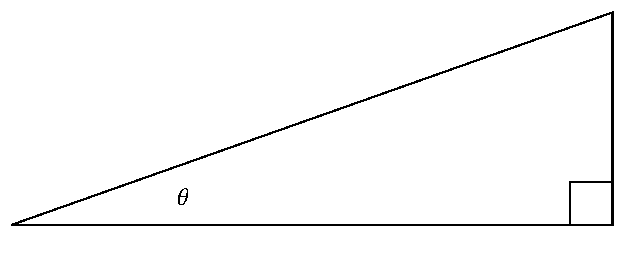
\includegraphics[height=2.8cm]{trig-substitution/pictures/08-03-ex5a.pdf}%
%}%
%\only<handout:0| 16>{%
%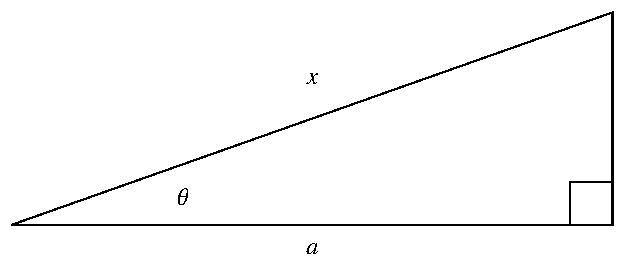
\includegraphics[height=2.8cm]{trig-substitution/pictures/08-03-ex5b.pdf}%
%}%
%\only<17->{%
%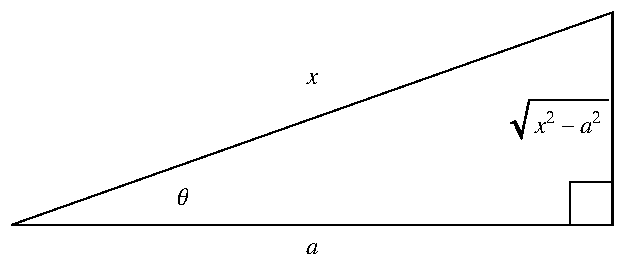
\includegraphics[height=2.8cm]{trig-substitution/pictures/08-03-ex5c.pdf}%
%}%
\end{center}
\end{columns}
\abovedisplayskip=0pt
\belowdisplayskip=0pt
\[
\uncover<2->{%
\alert<handout:0| 12>{%
\sqrt{\alert<handout:0| 7>{x^2}-a^2} =
}%
}%
\uncover<7->{%
\sqrt{\alert<handout:0| 7>{a^2\sec^2 \theta}-a^2} =
}%
\uncover<8->{%
\sqrt{a^2 \tan^2 \theta} =
}%
\uncover<9->{%
a |\tan  \theta | =
}%
\uncover<10->{%
\alert<handout:0| 12>{%
a \tan  \theta
}%
}%
\]
\abovedisplayskip=0pt
\belowdisplayskip=0pt
\begin{eqnarray*}
\uncover<11->{%
\int \frac{\alert<handout:0| 13>{\diff x}}{\alert<handout:0| 12>{\sqrt{x^2-a^2}}}%
}%
& \uncover<11->{ = } & %
\uncover<11->{%
\int\frac{\alert<handout:0| 13>{a\sec \theta \tan \theta \diff \theta}}{\alert<handout:0| 12>{a\tan \theta}}%
}%
\uncover<14->{%
 = \int \sec \theta \diff \theta
}\\%
& \uncover<15->{ = } & %
\uncover<15->{%
\ln | \alert<handout:0| 20>{\sec \theta} + \alert<handout:0| 18-19>{\tan \theta} | + C%
}  \uncover<19->{ = }  \uncover<19->{%
\ln \left| \alert<handout:0| 20>{\frac{x}{\alert<handout:0| 21>{a}}} + \alert<handout:0| 19>{\frac{\sqrt{x^2-a^2}}{\alert<handout:0| 21>{a}}}\right| + C
}\\%
& \uncover<21->{ = } & %
\uncover<21->{%
\ln \left| x + \sqrt{x^2 - a^2}\right| \only<handout:0| -22>{\alert<handout:0| 21-22>{- \ln a} \alert<handout:0| 22>{+ C}}\only<23->{\alert<handout:0| 23>{ + C_1}}%
}%
\end{eqnarray*}
\end{example}
\end{frame}
% end module trig-substitutions-ex5
